\documentclass[]{report}


% Title Page
\title{Homework II Solutions \\ of \\ \emph{Advanced Mechanical Vibrations} class.}
\author{Burak ER}

\usepackage{psfrag}

\usepackage{amsmath}

\usepackage{amssymb}

\usepackage{pstricks, pst-node, pst-plot, pst-circ}

\usepackage{moredefs}

\usepackage{hyperref}

\usepackage{cleveref}

\usepackage{graphicx}

\usepackage{epstopdf}

\usepackage{epsfig}

\usepackage{algorithm}

\usepackage{program}

\usepackage{graphicx}

\usepackage{caption}

\usepackage{subcaption}

\usepackage[autolinebreaks,useliterate]{mcode}

\crefname{lstlisting}{listing}{listings}

\Crefname{lstlisting}{Listing}{Listings}

\begin{document}


\maketitle
\begin{abstract}
Includes the solutions for the second homework problems of \emph{Advanced Mechanical Engineering} class given at Bursa Technical University, in fall semester 2013.
\\
\\
Written in \LaTeX ~markup language~using TeXstudio...
\end{abstract}
\section*{Problem 1}
Half-car model of a vehicle is given in the \cref{fig:2st_Assignment}. The physical properties are as follows: $m=420kg$, $m1=m2=53kg$, $I_x=820 kgm^2$, $b_1=0.7m$, $b_2=0.75m$, $k =10000Nm^{-1}$, $k_t=200000 Nm^{-1}$, $kR=25000 Nm^{-1}$, $k_4= 1972900 Nm^{-1}$, $c=200 Nsm^{-1}$. The vehicle is subject to base motions $y_1$ and $y_2$.

\begin{figure}[ht!]
\begin{subfigure}[b]{0.5\textwidth}
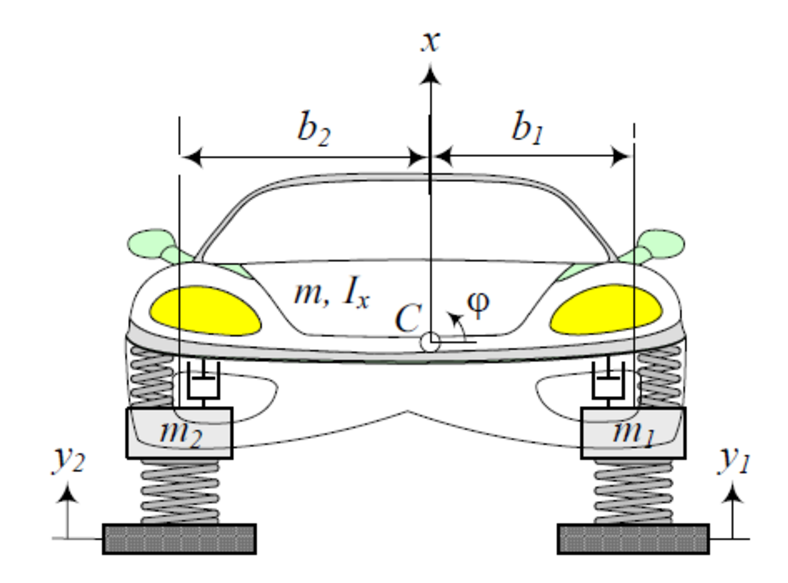
\includegraphics[width=\textwidth]{./Figures/2st_Assignment} \caption{whole car body}
\end{subfigure}~
\begin{subfigure}[b]{0.5\textwidth}
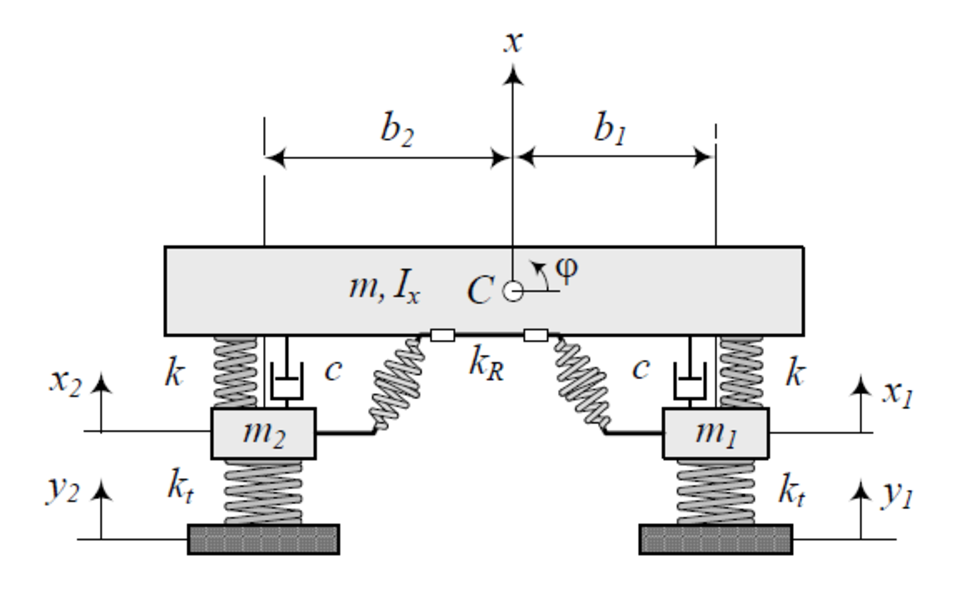
\includegraphics[width=\textwidth]{./Figures/2st_Assignment_1}
\caption{equivalent model}
\end{subfigure}
\caption{problem 1}
\label{fig:2st_Assignment}
\end{figure}
Mass, damping and stiffness matrices of the car model are
\begin{align*}
\mathbf{M}=\left[\begin{array}{cccc}
m&0&0&0\\
0&I_x&0&0 \\
0&0&m_1&0 \\
0&0&0&m_2
\end{array}\right]
\end{align*}

\begin{align*}
\mathbf{C}=\left[\begin{array}{cccc}
2c&cb_1-cb_2&-c&-c\\
cb_1-cb_2&cb_1^2+cb_2^2&-cb_1&cb_2 \\
-c&-cb_1&c&0 \\
-c&cb_2&0&c
\end{array}\right]
\end{align*}

\begin{align*}
\mathbf{K}=\left[\begin{array}{cccc}
2k&kb_1-kb_2&-k&-k\\
kb_1-kb_2&kb_1^2+kb_2^2&-kb_1&kb_2 \\
-k&-kb_1&k+k_t&0 \\
-k&kb_2&0&k+k_t
\end{array}\right]
\end{align*}

\subsection*{Question 1}

\begin{enumerate}
\item Find the undamped natural frequencies and vibration modes by
\begin{enumerate}
\item Solving characteristic polynomial.
\item Matrix iteration method.
\end{enumerate}
\item Plot the vibration modes, comment them and make conclusions.
\item Compute modal mass and stiffness values.
\item Show that vibration modes are orthogonal to each other with respect to mass and stiffness matrices.
\end{enumerate}

\begin{center}
\subsection*{Solution 1}
\end{center}
\textbf{Solving characteristic polynomial.}\\~\\
Undamped system characteristic polynominal is found from the equation
\begin{align*}
\mathrm{det}\left(-\lambda^2\mathbf{M}+ \mathbf{K}\right)=0
\end{align*}
which is found 
\begin{align*}
9.67\cdot 10^8\, \lambda^8 - 7.75\cdot 10^{12}\, \lambda^6 + 1.59\cdot 10^{16}\, \lambda^4 - 1.35\cdot 10^{18}\, \lambda^2 + 2.94\cdot 10^{19}=0
\end{align*}
where the solution of natural frequencies are found as
\begin{align*}
{\mathbf{\Lambda}}=\left[\begin{array}{c} 62.964\\ 62.951\\ 6.749\\6.517 \end{array}\right]\mathrm{radian/s}
\end{align*}
\emph{I}th mode shape of the system can be found by substituting $\lambda_i$ on the equation 
\begin{align*}
\left(-\lambda^2\mathbf{M}+ \mathbf{K}\right)\mathbf{u}=\mathbf{0}
\end{align*}
that is found 
\begin{align*}
\begin{array}{ccc} 500.0\, u_{2} + 10000.0\, u_{3} + 10000.0\, u_{4} + u_{1}\, \left(420.0\, \lambda_i^2 - 20000.0\right)= 0\\ 500.0\, u_{1} + 7000.0\, u_{3} - 7500.0\, u_{4} + u_{2}\, \left(820.0\, \lambda_i^2 - 35525.0\right)= 0\\ 10000.0\, u_{1} + 7000.0\, u_{2} + u_{3}\, \left(53.0\, \lambda_i^2 - 210000.0\right)= 0\\ 10000.0\, u_{1} - 7500.0\, u_{2} + u_{4}\, \left(53.0\, \lambda_i^2 - 210000.0\right)= 0 \end{array}
\end{align*}
with assuming $u_1=1$ and then normalizing the mode shapes, mode shapes are are found as\\~\\
for $\lambda_1$
\begin{align*}
\mathbf{u}_1=\left[\begin{array}{cccc} 0.00859  \\ 0.00011  \\ 0.97766  \\ 0.36874 \end{array}\right]
\end{align*}
for $\lambda_2$
\begin{align*}
\mathbf{u}_2=\left[\begin{array}{cccc} -0.00015  \\ 0.0031884  \\ -0.19903  \\ 0.92811 \end{array}\right]
\end{align*}
for $\lambda_3$
\begin{align*}
\mathbf{u}_3=\left[\begin{array}{cccc} -0.69795  \\ -0.71612 \\ 0.04038  \\ 0.04902\end{array}\right]
\end{align*}
for $\lambda_4$
\begin{align*}
\mathbf{u}_4=\left[\begin{array}{cccc} -0.71609 \\ 0.6979  \\ 0.05428  \\ -0.01575 \end{array}\right]
\end{align*}
\\~\\
\textbf{Plot the vibration modes, comment them and make conclusions.}
\\~\\
Plot of vibration modes is given in \cref{fig:allmodes}. What can be seen from the figure is; the dominant term in the first and second mode are displacements of the tires. These modes have two highest natural frequencies. In the third and fourth mode the dominant variables are displacement and the rotation of the car body. These modes have the lowest two natural frequencies.
\\~\\
It is concluded that, as expected, low frequency modes exist just because of the contribution of the body of the car and high frequency modes exist because of the contribution of the tires.
\begin{figure}[h!]
\centering
% This file is generated by the MATLAB m-file laprint.m. It can be included
% into LaTeX documents using the packages graphicx, color and psfrag.
% It is accompanied by a postscript file. A sample LaTeX file is:
%    \documentclass{article}\usepackage{graphicx,color,psfrag}
%    \begin{document}% This file is generated by the MATLAB m-file laprint.m. It can be included
% into LaTeX documents using the packages graphicx, color and psfrag.
% It is accompanied by a postscript file. A sample LaTeX file is:
%    \documentclass{article}\usepackage{graphicx,color,psfrag}
%    \begin{document}% This file is generated by the MATLAB m-file laprint.m. It can be included
% into LaTeX documents using the packages graphicx, color and psfrag.
% It is accompanied by a postscript file. A sample LaTeX file is:
%    \documentclass{article}\usepackage{graphicx,color,psfrag}
%    \begin{document}\input{allmode}\end{document}
% See http://www.mathworks.de/matlabcentral/fileexchange/loadFile.do?objectId=4638
% for recent versions of laprint.m.
%
% created by:           LaPrint version 3.16 (13.9.2004)
% created on:           05-Jan-2014 21:04:15
% eps bounding box:     15 cm x 8.8506 cm
% comment:              
%
\begin{psfrags}%
\psfragscanon%
%
% text strings:
\psfrag{s01}[b][b]{\color[rgb]{0,0,0}\setlength{\tabcolsep}{0pt}\begin{tabular}{c}mode 1\\62.964 rad/sn\end{tabular}}%
\psfrag{s02}[b][b]{\color[rgb]{0,0,0}\setlength{\tabcolsep}{0pt}\begin{tabular}{c}relative displacement\end{tabular}}%
\psfrag{s05}[b][b]{\color[rgb]{0,0,0}\setlength{\tabcolsep}{0pt}\begin{tabular}{c}mode 3\\6.749[rad/sn]\end{tabular}}%
\psfrag{s07}[b][b]{\color[rgb]{0,0,0}\setlength{\tabcolsep}{0pt}\begin{tabular}{c}relative displacement\end{tabular}}%
\psfrag{s09}[b][b]{\color[rgb]{0,0,0}\setlength{\tabcolsep}{0pt}\begin{tabular}{c}mode 4\\6.517[rad/sn]\end{tabular}}%
\psfrag{s11}[b][b]{\color[rgb]{0,0,0}\setlength{\tabcolsep}{0pt}\begin{tabular}{c}relative displacement\end{tabular}}%
\psfrag{s13}[b][b]{\color[rgb]{0,0,0}\setlength{\tabcolsep}{0pt}\begin{tabular}{c}mode 2\\62.951[rad/sn]\end{tabular}}%
\psfrag{s15}[b][b]{\color[rgb]{0,0,0}\setlength{\tabcolsep}{0pt}\begin{tabular}{c}relative displacement\end{tabular}}%
%
% xticklabels:
\psfrag{x01}[t][t]{0}%
\psfrag{x02}[t][t]{0.1}%
\psfrag{x03}[t][t]{0.2}%
\psfrag{x04}[t][t]{0.3}%
\psfrag{x05}[t][t]{0.4}%
\psfrag{x06}[t][t]{0.5}%
\psfrag{x07}[t][t]{0.6}%
\psfrag{x08}[t][t]{0.7}%
\psfrag{x09}[t][t]{0.8}%
\psfrag{x10}[t][t]{0.9}%
\psfrag{x11}[t][t]{1}%
\psfrag{x12}[t][t]{1}%
\psfrag{x13}[t][t]{1.5}%
\psfrag{x14}[t][t]{2}%
\psfrag{x15}[t][t]{2.5}%
\psfrag{x16}[t][t]{3}%
\psfrag{x17}[t][t]{3.5}%
\psfrag{x18}[t][t]{4}%
\psfrag{x19}[t][t]{1}%
\psfrag{x20}[t][t]{2}%
\psfrag{x21}[t][t]{3}%
\psfrag{x22}[t][t]{4}%
\psfrag{x23}[t][t]{1}%
\psfrag{x24}[t][t]{2}%
\psfrag{x25}[t][t]{3}%
\psfrag{x26}[t][t]{4}%
\psfrag{x27}[t][t]{1}%
\psfrag{x28}[t][t]{2}%
\psfrag{x29}[t][t]{3}%
\psfrag{x30}[t][t]{4}%
%
% yticklabels:
\psfrag{v01}[r][r]{0}%
\psfrag{v02}[r][r]{0.1}%
\psfrag{v03}[r][r]{0.2}%
\psfrag{v04}[r][r]{0.3}%
\psfrag{v05}[r][r]{0.4}%
\psfrag{v06}[r][r]{0.5}%
\psfrag{v07}[r][r]{0.6}%
\psfrag{v08}[r][r]{0.7}%
\psfrag{v09}[r][r]{0.8}%
\psfrag{v10}[r][r]{0.9}%
\psfrag{v11}[r][r]{1}%
\psfrag{v12}[r][r]{-1}%
\psfrag{v13}[r][r]{-0.5}%
\psfrag{v14}[r][r]{0}%
\psfrag{v15}[r][r]{0.5}%
\psfrag{v16}[r][r]{1}%
\psfrag{v17}[r][r]{-1}%
\psfrag{v18}[r][r]{-0.5}%
\psfrag{v19}[r][r]{0}%
\psfrag{v20}[r][r]{0.5}%
\psfrag{v21}[r][r]{1}%
\psfrag{v22}[r][r]{-1}%
\psfrag{v23}[r][r]{-0.5}%
\psfrag{v24}[r][r]{0}%
\psfrag{v25}[r][r]{0.5}%
\psfrag{v26}[r][r]{1}%
\psfrag{v27}[r][r]{-1}%
\psfrag{v28}[r][r]{-0.5}%
\psfrag{v29}[r][r]{0}%
\psfrag{v30}[r][r]{0.5}%
\psfrag{v31}[r][r]{1}%
%
% Figure:
\resizebox{10cm}{!}{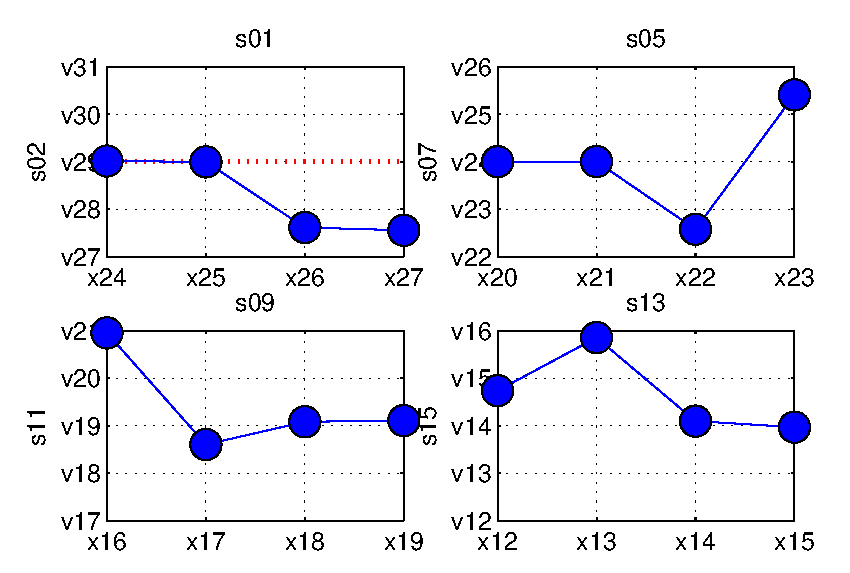
\includegraphics{./Figures/allmode.eps}}%
\end{psfrags}%
%
% End allmode.tex
\end{document}
% See http://www.mathworks.de/matlabcentral/fileexchange/loadFile.do?objectId=4638
% for recent versions of laprint.m.
%
% created by:           LaPrint version 3.16 (13.9.2004)
% created on:           05-Jan-2014 21:04:15
% eps bounding box:     15 cm x 8.8506 cm
% comment:              
%
\begin{psfrags}%
\psfragscanon%
%
% text strings:
\psfrag{s01}[b][b]{\color[rgb]{0,0,0}\setlength{\tabcolsep}{0pt}\begin{tabular}{c}mode 1\\62.964 rad/sn\end{tabular}}%
\psfrag{s02}[b][b]{\color[rgb]{0,0,0}\setlength{\tabcolsep}{0pt}\begin{tabular}{c}relative displacement\end{tabular}}%
\psfrag{s05}[b][b]{\color[rgb]{0,0,0}\setlength{\tabcolsep}{0pt}\begin{tabular}{c}mode 3\\6.749[rad/sn]\end{tabular}}%
\psfrag{s07}[b][b]{\color[rgb]{0,0,0}\setlength{\tabcolsep}{0pt}\begin{tabular}{c}relative displacement\end{tabular}}%
\psfrag{s09}[b][b]{\color[rgb]{0,0,0}\setlength{\tabcolsep}{0pt}\begin{tabular}{c}mode 4\\6.517[rad/sn]\end{tabular}}%
\psfrag{s11}[b][b]{\color[rgb]{0,0,0}\setlength{\tabcolsep}{0pt}\begin{tabular}{c}relative displacement\end{tabular}}%
\psfrag{s13}[b][b]{\color[rgb]{0,0,0}\setlength{\tabcolsep}{0pt}\begin{tabular}{c}mode 2\\62.951[rad/sn]\end{tabular}}%
\psfrag{s15}[b][b]{\color[rgb]{0,0,0}\setlength{\tabcolsep}{0pt}\begin{tabular}{c}relative displacement\end{tabular}}%
%
% xticklabels:
\psfrag{x01}[t][t]{0}%
\psfrag{x02}[t][t]{0.1}%
\psfrag{x03}[t][t]{0.2}%
\psfrag{x04}[t][t]{0.3}%
\psfrag{x05}[t][t]{0.4}%
\psfrag{x06}[t][t]{0.5}%
\psfrag{x07}[t][t]{0.6}%
\psfrag{x08}[t][t]{0.7}%
\psfrag{x09}[t][t]{0.8}%
\psfrag{x10}[t][t]{0.9}%
\psfrag{x11}[t][t]{1}%
\psfrag{x12}[t][t]{1}%
\psfrag{x13}[t][t]{1.5}%
\psfrag{x14}[t][t]{2}%
\psfrag{x15}[t][t]{2.5}%
\psfrag{x16}[t][t]{3}%
\psfrag{x17}[t][t]{3.5}%
\psfrag{x18}[t][t]{4}%
\psfrag{x19}[t][t]{1}%
\psfrag{x20}[t][t]{2}%
\psfrag{x21}[t][t]{3}%
\psfrag{x22}[t][t]{4}%
\psfrag{x23}[t][t]{1}%
\psfrag{x24}[t][t]{2}%
\psfrag{x25}[t][t]{3}%
\psfrag{x26}[t][t]{4}%
\psfrag{x27}[t][t]{1}%
\psfrag{x28}[t][t]{2}%
\psfrag{x29}[t][t]{3}%
\psfrag{x30}[t][t]{4}%
%
% yticklabels:
\psfrag{v01}[r][r]{0}%
\psfrag{v02}[r][r]{0.1}%
\psfrag{v03}[r][r]{0.2}%
\psfrag{v04}[r][r]{0.3}%
\psfrag{v05}[r][r]{0.4}%
\psfrag{v06}[r][r]{0.5}%
\psfrag{v07}[r][r]{0.6}%
\psfrag{v08}[r][r]{0.7}%
\psfrag{v09}[r][r]{0.8}%
\psfrag{v10}[r][r]{0.9}%
\psfrag{v11}[r][r]{1}%
\psfrag{v12}[r][r]{-1}%
\psfrag{v13}[r][r]{-0.5}%
\psfrag{v14}[r][r]{0}%
\psfrag{v15}[r][r]{0.5}%
\psfrag{v16}[r][r]{1}%
\psfrag{v17}[r][r]{-1}%
\psfrag{v18}[r][r]{-0.5}%
\psfrag{v19}[r][r]{0}%
\psfrag{v20}[r][r]{0.5}%
\psfrag{v21}[r][r]{1}%
\psfrag{v22}[r][r]{-1}%
\psfrag{v23}[r][r]{-0.5}%
\psfrag{v24}[r][r]{0}%
\psfrag{v25}[r][r]{0.5}%
\psfrag{v26}[r][r]{1}%
\psfrag{v27}[r][r]{-1}%
\psfrag{v28}[r][r]{-0.5}%
\psfrag{v29}[r][r]{0}%
\psfrag{v30}[r][r]{0.5}%
\psfrag{v31}[r][r]{1}%
%
% Figure:
\resizebox{10cm}{!}{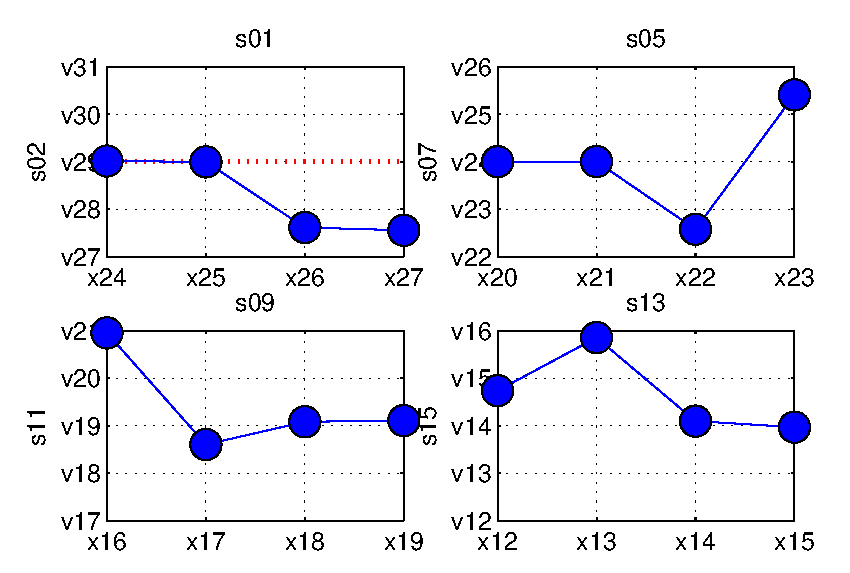
\includegraphics{./Figures/allmode.eps}}%
\end{psfrags}%
%
% End allmode.tex
\end{document}
% See http://www.mathworks.de/matlabcentral/fileexchange/loadFile.do?objectId=4638
% for recent versions of laprint.m.
%
% created by:           LaPrint version 3.16 (13.9.2004)
% created on:           05-Jan-2014 21:04:15
% eps bounding box:     15 cm x 8.8506 cm
% comment:              
%
\begin{psfrags}%
\psfragscanon%
%
% text strings:
\psfrag{s01}[b][b]{\color[rgb]{0,0,0}\setlength{\tabcolsep}{0pt}\begin{tabular}{c}mode 1\\62.964 rad/sn\end{tabular}}%
\psfrag{s02}[b][b]{\color[rgb]{0,0,0}\setlength{\tabcolsep}{0pt}\begin{tabular}{c}relative displacement\end{tabular}}%
\psfrag{s05}[b][b]{\color[rgb]{0,0,0}\setlength{\tabcolsep}{0pt}\begin{tabular}{c}mode 3\\6.749[rad/sn]\end{tabular}}%
\psfrag{s07}[b][b]{\color[rgb]{0,0,0}\setlength{\tabcolsep}{0pt}\begin{tabular}{c}relative displacement\end{tabular}}%
\psfrag{s09}[b][b]{\color[rgb]{0,0,0}\setlength{\tabcolsep}{0pt}\begin{tabular}{c}mode 4\\6.517[rad/sn]\end{tabular}}%
\psfrag{s11}[b][b]{\color[rgb]{0,0,0}\setlength{\tabcolsep}{0pt}\begin{tabular}{c}relative displacement\end{tabular}}%
\psfrag{s13}[b][b]{\color[rgb]{0,0,0}\setlength{\tabcolsep}{0pt}\begin{tabular}{c}mode 2\\62.951[rad/sn]\end{tabular}}%
\psfrag{s15}[b][b]{\color[rgb]{0,0,0}\setlength{\tabcolsep}{0pt}\begin{tabular}{c}relative displacement\end{tabular}}%
%
% xticklabels:
\psfrag{x01}[t][t]{0}%
\psfrag{x02}[t][t]{0.1}%
\psfrag{x03}[t][t]{0.2}%
\psfrag{x04}[t][t]{0.3}%
\psfrag{x05}[t][t]{0.4}%
\psfrag{x06}[t][t]{0.5}%
\psfrag{x07}[t][t]{0.6}%
\psfrag{x08}[t][t]{0.7}%
\psfrag{x09}[t][t]{0.8}%
\psfrag{x10}[t][t]{0.9}%
\psfrag{x11}[t][t]{1}%
\psfrag{x12}[t][t]{1}%
\psfrag{x13}[t][t]{1.5}%
\psfrag{x14}[t][t]{2}%
\psfrag{x15}[t][t]{2.5}%
\psfrag{x16}[t][t]{3}%
\psfrag{x17}[t][t]{3.5}%
\psfrag{x18}[t][t]{4}%
\psfrag{x19}[t][t]{1}%
\psfrag{x20}[t][t]{2}%
\psfrag{x21}[t][t]{3}%
\psfrag{x22}[t][t]{4}%
\psfrag{x23}[t][t]{1}%
\psfrag{x24}[t][t]{2}%
\psfrag{x25}[t][t]{3}%
\psfrag{x26}[t][t]{4}%
\psfrag{x27}[t][t]{1}%
\psfrag{x28}[t][t]{2}%
\psfrag{x29}[t][t]{3}%
\psfrag{x30}[t][t]{4}%
%
% yticklabels:
\psfrag{v01}[r][r]{0}%
\psfrag{v02}[r][r]{0.1}%
\psfrag{v03}[r][r]{0.2}%
\psfrag{v04}[r][r]{0.3}%
\psfrag{v05}[r][r]{0.4}%
\psfrag{v06}[r][r]{0.5}%
\psfrag{v07}[r][r]{0.6}%
\psfrag{v08}[r][r]{0.7}%
\psfrag{v09}[r][r]{0.8}%
\psfrag{v10}[r][r]{0.9}%
\psfrag{v11}[r][r]{1}%
\psfrag{v12}[r][r]{-1}%
\psfrag{v13}[r][r]{-0.5}%
\psfrag{v14}[r][r]{0}%
\psfrag{v15}[r][r]{0.5}%
\psfrag{v16}[r][r]{1}%
\psfrag{v17}[r][r]{-1}%
\psfrag{v18}[r][r]{-0.5}%
\psfrag{v19}[r][r]{0}%
\psfrag{v20}[r][r]{0.5}%
\psfrag{v21}[r][r]{1}%
\psfrag{v22}[r][r]{-1}%
\psfrag{v23}[r][r]{-0.5}%
\psfrag{v24}[r][r]{0}%
\psfrag{v25}[r][r]{0.5}%
\psfrag{v26}[r][r]{1}%
\psfrag{v27}[r][r]{-1}%
\psfrag{v28}[r][r]{-0.5}%
\psfrag{v29}[r][r]{0}%
\psfrag{v30}[r][r]{0.5}%
\psfrag{v31}[r][r]{1}%
%
% Figure:
\resizebox{10cm}{!}{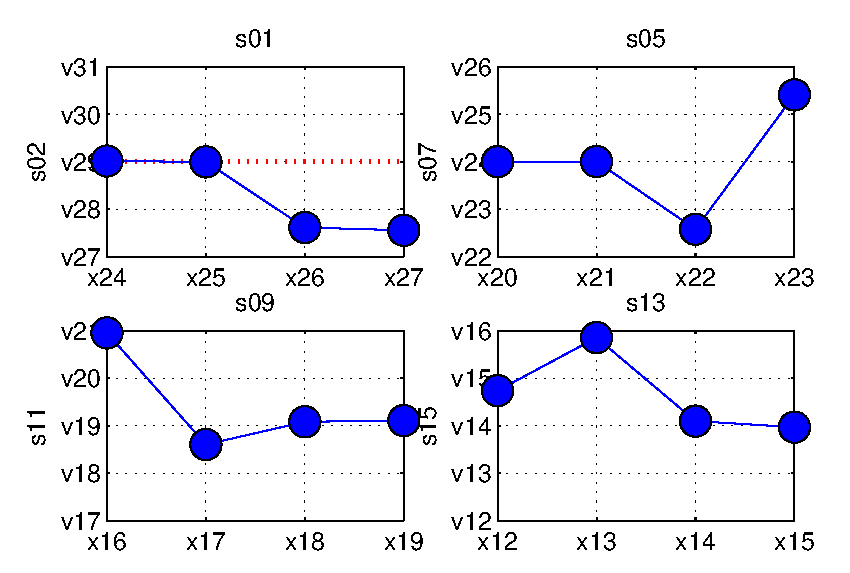
\includegraphics{./Figures/allmode.eps}}%
\end{psfrags}%
%
% End allmode.tex

\caption{Vibration modes}
\label{fig:allmodes}
\end{figure}
\newpage
~\\
\textbf{Compute modal mass and stiffness matrices.}
\\~\\
Modal mass and stiffness matrices are found from the relations
\begin{align*}
\mathbf{m}=\mathbf{\Phi}^T \mathbf{M} \mathbf{\Phi} \\
\mathbf{k}=\mathbf{\Phi}^T \mathbf{K} \mathbf{\Phi}
\end{align*}
where $\mathbf{\Phi}$ is the eigen modes matrix. If we calculate them it is found that
\begin{align*}
\mathbf{m}=\left(\begin{array}{cccc} 53.0 & 0 & 0 & 0\\ 0 & 53.0 & 0 & 0\\ 0 & 0 & 434.0 & 0\\ 0 & 0 & 0 & 764.0 \end{array}\right)
\end{align*}
and
\begin{align*}
\mathbf{k}=\left(\begin{array}{cccc} 2.1\cdot 10^5 & 0 & 0 & 0\\ 0 & 2.1\cdot 10^5 & 0 & 0\\ 0 & 0 & 1.98\cdot 10^4 & 0\\ 0 & 0 & 0 & 3.24\cdot 10^4 \end{array}\right)
\end{align*}
\newpage
~\\
\textbf{Show that vibration modes are orthogonal to each other with respect to mass and stiffness matrices.}
\\~\\
Zero bidiagonal elements in modal and stiffness matrices mean that the modes are orthogonal to each other with respect to mass and stiffness matrices. It is already showed that they are equal to zero in the previous answer.
\subsection*{Question 2}
\textbf{Suppose that while moving with a speed $\mathrm{V} = 60 km/h$ the right tire passes over a half sine wave-like bump on the road as shown below, where $\mathrm{a} = 30cm$ and $\mathrm{b} = 5cm$. Assuming zero initial conditions plot the 5 seconds responses of the coordinates $x_1$ and $x_2$.}
\begin{center}
\subsection*{Solution 2}
\end{center}
This problem can be solved numerically integrating the equations of motion. Before we do that, applied force on the second tire should be calculated. The force on the tire depends on the displacement of the road. Therefore, displacement profile with respect to time is
\begin{align*}
\mathrm{T}& =0.072\frac{\mathrm{a}}{\mathrm{V}}\quad \mathrm{(seconds)}
\end{align*}
\begin{align*}
y_2& =\{\begin{array}{clc}
\mathrm{b}\sin\left(\frac{2\pi}{\mathrm{T}}t\right) &,& 0\leq t \leq \frac{\mathrm{T}}{2} \\ 
0 &,& \frac{\mathrm{T}}{2}<t
\end{array}
\end{align*}
with the found displacement of the road, complete force vector of the model is found as
\begin{align*}
\mathrm{F}& =\left[\begin{array}{ccc}
0\\
0\\
y_1 k_t\\
y_2 k_t
\end{array}\right]
\end{align*}
With this calculated road input force, a numerical solution to the equations of motion of the car is done by a matlab function. This function is given in~\cref{lst:odefunc} and it calculates required derivatives of the system by using order reducing method. The derivatives can be integrated by a numerical method, for example Runge-Kutta. For the integration of derivatives \mcode{Ode45} function of matlab is used in which integration is done with Runge-Kutta45 method. Integration is completed with the command in \cref{lst:command}.
\lstset{frame=single,numbers=left}
\begin{lstlisting}[label=lst:command,caption=integration commands]
options = odeset('MaxStep',1e-3)
[t y]=ode45(@odefunc,[0 5],[0 0 0 0 0 0 0 0],options);
\end{lstlisting}
%\begin{align*}
%{{\mathbf M}}\mathbf{\ddot {\mathbf x}}+{{\mathbf C}}\mathbf{\dot {\mathbf x}}+{{\mathbf K}}\mathbf{ {\mathbf x}}={{\mathbf F}}
%\end{align*}
\newpage
\lstset{frame=single,numbers=left}
\lstinputlisting[label=lst:odefunc,caption={{odefunc.m}}]{Matlab/odefunc.m}
Using \cref{lst:command} with \cref{lst:odefunc} the resulting time dependent behaviors of the displacements of the right and the left tires are given in \cref{fig:timedependenttires}.
\begin{figure}[ht!]
\centering
\input{./Figures/timedependent}
\caption{Time dependent motion of the tires of the car.}
\label{fig:timedependenttires}
\end{figure}

\section*{Problem 2}
In \cref{fig:problem2}, a beam  with fixed one end, carrying  a rigid tip mass M , and exhibits transverse vibrations is given. Physical properties are as follows:  $L =1m$, $E=210GPa$, $\rho=7800kgm^{-3}$, sizes of the rectangular cross section $a=2cm$ $b=1cm$, $M$ is twice of the beam mass.
\begin{figure}[ht!]
\centering
\includegraphics[width=\textwidth]{./Figures/2st_Assignment_2}
\caption{Problem 2}
\label{fig:problem2}
\end{figure}
\subsection*{Question 1}
\textbf{Derive the equations of motion with suitable boundary conditions.}
\begin{center}
\subsection*{Solution 1}
\end{center}
The transverse equation of motion for the beam is given by
\begin{align*}
 EI~\cfrac{\partial^4 w}{\partial x^4} + \rho A~\cfrac{\partial^2 w}{\partial t^2} = 0
\end{align*}
The boundary conditions for the problem are as follows:\\
\begin{enumerate}
\item {zero displacement at $x=0$ :\\ \begin{align*}
w\left(0,t\right)=0
\end{align*} }
\item {zero slope of displacement at $x=0$ :\\ \begin{align*}
\cfrac{\partial w\left(0,t\right)}{\partial x}=0
\end{align*} }
\item {shear force acceleration of lumped mass equilibrium at $x=L$ :\\ \begin{align*}
 EI~\cfrac{\partial w^3\left(L,t\right)}{\partial x^3}=M\cfrac{\partial w^2\left(L,t\right)}{\partial t^2}
\end{align*} }
\item {zero moment at $x=L$ :\\ \begin{align*}
 EI~\cfrac{\partial w^2\left(L,t\right)}{\partial x^2}=0
\end{align*} }
\end{enumerate}
\subsection*{Question 2}
\textbf{Find the first five natural frequencies (Hz) and vibration modes of the system. Plot the vibration modes in the same figure.}
\begin{center}
\subsection*{Solution 2}
\end{center}
Using seperation of variables method, the displacements of the beam can be written as
\begin{align}
u\left(x,t\right)=U\left(x\right)T\left(t\right)
\end{align}
using this assumption with the equations of motion we have
\begin{align}
U^{IV} -\lambda^4U=0\\
\ddot{T} +\omega^2 T=0
\end{align}
Using these differential equations , the space dependent part of the solution of transverse vibration of beam is found as
\begin{equation}
X(x)=A\cosh\left(\lambda x\right)+B\sinh\left(\lambda x\right)+C\cos\left(\lambda x\right)+D\sin\left(\lambda x\right)
\label{eq:spacesolution}
\end{equation}
and time dependent part as
\begin{equation*}
T(t)=\bar{A}\cos\left({\omega t}\right)+\bar{B}\sin\left({\omega t}\right)
\end{equation*}
where $\omega^2=\lambda^4 \cfrac{EI}{\rho A}$. In these equations there are 4 variables to determine in the space dependent part. Using boundary conditions, these variables can be determined. Using first two boundary conditions
\begin{equation}
U\left(0,t\right)= 0 \quad ; \quad  A+C=0 \quad \Longrightarrow \quad A=-C \label{eq:acrel}
\end{equation}
\begin{equation}
U'\left(0,t\right)= 0\quad ; \quad B+D=0 \quad \Longrightarrow \quad B=-D\label{eq:bdrel}
\end{equation}
Using other boundary conditions
\begin{align*}
EIU''\left(L,t\right)= 0&; \lambda^2 \biggl(A\cosh\left(\lambda L\right)+B\sinh\left(\lambda L\right)\\
&-C\cos\left(\lambda L\right) -D\sin\left(\lambda L\right)\biggr)=0\\
EIU'''\left(L,t\right)-M\omega^2U\left(L,t\right)= 0&; EI \lambda^3\biggl(A\sinh\left(\lambda L\right)+B\cosh\left(\lambda L\right)\\&+C\sin\left(\lambda L\right)-D\cos\left(\lambda L\right)\biggr)\\
&- M\omega^2\biggl(A\cosh\left(\lambda L\right)+B\sinh\left(\lambda L\right)\\&+C\cos\left(\lambda L\right)+D\sin\left(\lambda L\right) \biggr)
\end{align*}
from the third boundary condition we have
\begin{equation}
B=-\cfrac{\cosh\left(\lambda L\right)+\cos\left(\lambda L\right)}{\sinh\left(\lambda L\right)+\sin\left(\lambda L\right)}A
\label{eq:barel}
\end{equation}
using all relations in the fourth boundary condition it is found that
\begin{align*}
A\biggl[\lambda^3\left( \sinh\!\left(L\, \lambda\right)-\sin\!\left(L\, \lambda\right)  - \frac{{\cos\!\left(L\, \lambda\right) + \cosh\!\left(L\, \lambda\right)}}{\sin\!\left(L\, \lambda\right) + \sinh\!\left(L\, \lambda\right)}{\left(\cos\!\left(L\, \lambda\right) + \cosh\!\left(L\, \lambda\right)\right)}\right)-&
\\ 
\frac{M\, {\lambda}^4\,}{{ \mathrm{\rho}\, A}} \left(\cosh\!\left(L\, \lambda\right) - \cos\!\left(L\, \lambda\right) + \frac{\cos\!\left(L\, \lambda\right) + \cosh\!\left(L\, \lambda\right)\, }{\sin\!\left(L\, \lambda\right) + \sinh\!\left(L\, \lambda\right)}\left(\sin\!\left(L\, \lambda\right) - \sinh\!\left(L\, \lambda\right)\right)\right)\biggr]&\\= 0&
\end{align*}
where for a non trivial solution $A\neq 0$ should be satisfied. Therefore, the expression inside the brackets must be zero. This results an equation in terms of $\lambda$ where solution corresponds to the eigen frequencies of the beam. 
\\~\\
Since it is impossible to obtain explicit expression for the $\lambda$, numerical solution is done. Therefore, the first five space frequencies are found as

\begin{align*}
\mathbf{\mathrm{\Lambda}}=\left[\begin{array}{c} 3.8614\\ 7.0316\\ 10.1850\\ 13.3326\\ 16.4779 \end{array}\right] \mathrm{rad/m}
\end{align*}
The first five natural frequencies that are found  as
\begin{align*}
\mathbf{\mathrm{\Omega}}=\left[\begin{array}{c} 223.3469\\ 740.6028\\ 1553.8015\\ 2662.5970\\ 4067.0401 \end{array}
\right] \mathrm{Hz}
\end{align*}
Mode shape that corresponds to an arbitrary $\lambda_r$ is found from ~\cref{eq:spacesolution} using the relations \crefrange{eq:acrel}{eq:barel}. The expression for the mode shapes for a specific $\lambda$ is found as
\begin{align*}
U_r\left(x\right)&= A\biggl[\cosh\!\left(\lambda_r\, x\right) - \cos\!\left(\lambda_r\, x\right) +\left(\sin\!\left(\lambda_r\, x\right)\,- \sinh\!\left(\lambda_r\, x\right)\,\right)\\&\quad \quad \frac{ \left(\cos\!\left(L\, \lambda_r\right) + \cosh\!\left(L\, \lambda_r\right)\right)}{\sin\!\left(L\, \lambda_r\right) + \sinh\!\left(L\, \lambda_r\right)}\biggr]
\end{align*}
The plot of the first five modes' shapes $U_r\left(x\right)$ is given in \cref{fig:cantileverallmodes}.
\begin{figure}[ht!]
\centering
\input{./Figures/cantileverallmodes}
\caption{First five vibration modes of the beam with a tip mass. }
\label{fig:cantileverallmodes}
\end{figure}
\newpage
\subsection*{Question 3}
\textbf{Assume that  M=0, and   an impulse force with magnitude 10N is applied on the tip at t =0. Plot  the shape of the beam after 1, 3, and 5 seconds.}
\\~\\
For this problem setting $M=0$ gives
\begin{align*}
EI \lambda^3\biggl(A\sinh\left(\lambda L\right)+B\cosh\left(\lambda L\right)+C\sin\left(\lambda L\right)-D\cos\left(\lambda L\right)\biggr)=0
\end{align*}
for the last boundary condition. Using other boundary conditions 
the frequency equation is found as
\begin{align*}
\sinh\left(\lambda L\right)-\sin\left(\lambda L\right)- \frac{ \left(\cos\!\left(L\, \lambda\right) + \cosh\!\left(L\, \lambda\right)\right)}{\sin\!\left(L\, \lambda\right) + \sinh\!\left(L\, \lambda\right)}\left(\cosh\left(\lambda L\right)+\cos\left(\lambda L\right)\right)=0
\end{align*}
Again using a numerical solution procedure, possible $\lambda$ values can be determined. Using found frequencies in the \cref{eq:spacesolution} explicit form of $U\left(x\right)$ is written as
\begin{equation}
\begin{split}
U_r\left(x\right)&= A\biggl[\cosh\!\left(\lambda_r\, x\right) - \cos\!\left(\lambda_r\, x\right) +\left(\sin\!\left(\lambda_r\, x\right)\,- \sinh\!\left(\lambda_r\, x\right)\,\right)\\&\quad \quad \frac{ \left(\cos\!\left(L\, \lambda_r\right) + \cosh\!\left(L\, \lambda_r\right)\right)}{\sin\!\left(L\, \lambda_r\right) + \sinh\!\left(L\, \lambda_r\right)}\biggr]
\end{split}
\label{equ:uexpression}
\end{equation}
which is going to be used for the forced response of the system.
\\~\\
Forced response of the system can be written in modal coordinates as
\begin{align}
u\left(x,t\right)=\sum_{r=0}^{r=\infty}U_r\left(x\right)\eta_r\left(t\right)
\label{equ:forcedassumption}
\end{align}
using this form in the equation of motion and multpliying both sides with the mode shape for arbitrary $\lambda_r$ for the beam and using the orthogonality conditions of the different mode shapes it is found that
\begin{align}
\ddot{\eta}_r\left(t\right)+\omega_r^2\eta_r\left(t\right)=F_r\left(t\right)\label{equ:modalequationsofmotion}
\end{align}
where 
\begin{equation}
F_r\left(t\right)=\int_{0}^{L}U_r\left(x\right)f\left(x,t\right)\;dx
\label{equ:modalforce}
\end{equation}
here $f\left(x,t\right)=f_0\delta\left(x-L\right)\delta\left(t\right)$ for the problem. Using \cref{equ:uexpression} in \cref{equ:modalforce} we find
\begin{equation}
\begin{split}
F_r\left(t\right)=U_r\left(L\right) f_{0}\, \delta\!\left(t\right)\,
\end{split}
\label{equ:modalforceexplicit}
\end{equation}
For the time evolution of the system we should solve \cref{equ:modalequationsofmotion}. General solution to \cref{equ:modalequationsofmotion} without initial conditions is given as
\begin{equation}
\eta_r\left(t\right)=\cfrac{1}{\omega_r}\int_{0}^{t} F_r\left(t-\tau\right)\sin\left(\omega_r\tau\right)d\tau
\end{equation}
using \cref{equ:modalforceexplicit} it is found that
\begin{equation}
\eta_r\left(t\right)=\frac{U_r\left(L\right) f_{0}\,}{\omega_r}\sin\left(\omega_r t\right)
\label{equ:etaexplicit}
\end{equation}
\Cref{equ:etaexplicit} with \crefrange{equ:uexpression}{equ:forcedassumption} completely describes the forced response of the beam. Time evolution of the system requires to combine multiple modes together, therefore, it will change its behavior as more modes are added into the solution. Usually maximum number of modes that are required for an accurate solution is found by tracking the convergence of the solution while changing included number of modes. Plots of the time evolution of the beam at t=1,3,5 s using different number of modes is given in \cref{fig:cantilevertimeevolution}.
\begin{figure}[ht!]

\end{figure}
\begin{figure}[ht!]
\begin{subfigure}[b]{0.5\textwidth}
\centering
% This file is generated by the MATLAB m-file laprint.m. It can be included
% into LaTeX documents using the packages graphicx, color and psfrag.
% It is accompanied by a postscript file. A sample LaTeX file is:
%    \documentclass{article}\usepackage{graphicx,color,psfrag}
%    \begin{document}% This file is generated by the MATLAB m-file laprint.m. It can be included
% into LaTeX documents using the packages graphicx, color and psfrag.
% It is accompanied by a postscript file. A sample LaTeX file is:
%    \documentclass{article}\usepackage{graphicx,color,psfrag}
%    \begin{document}% This file is generated by the MATLAB m-file laprint.m. It can be included
% into LaTeX documents using the packages graphicx, color and psfrag.
% It is accompanied by a postscript file. A sample LaTeX file is:
%    \documentclass{article}\usepackage{graphicx,color,psfrag}
%    \begin{document}\input{cantilevertimeevolution_t=all}\end{document}
% See http://www.mathworks.de/matlabcentral/fileexchange/loadFile.do?objectId=4638
% for recent versions of laprint.m.
%
% created by:           LaPrint version 3.16 (13.9.2004)
% created on:           14-Jan-2014 00:37:06
% eps bounding box:     15 cm x 10.0472 cm
% comment:              
%
\begin{psfrags}%
\psfragscanon%
%
% text strings:
\psfrag{s01}[t][t]{\color[rgb]{0,0,0}\setlength{\tabcolsep}{0pt}\begin{tabular}{c}{x}\end{tabular}}%
\psfrag{s02}[b][b]{\color[rgb]{0,0,0}\setlength{\tabcolsep}{0pt}\begin{tabular}{c}t=5 s\end{tabular}}%
\psfrag{s03}[b][b]{\color[rgb]{0,0,0}\setlength{\tabcolsep}{0pt}\begin{tabular}{c}displacement [m]\end{tabular}}%
\psfrag{s06}[][]{\color[rgb]{0,0,0}\setlength{\tabcolsep}{0pt}\begin{tabular}{c} \end{tabular}}%
\psfrag{s07}[][]{\color[rgb]{0,0,0}\setlength{\tabcolsep}{0pt}\begin{tabular}{c} \end{tabular}}%
\psfrag{s08}[t][t]{\color[rgb]{0,0,0}\setlength{\tabcolsep}{0pt}\begin{tabular}{c}{x}\end{tabular}}%
\psfrag{s09}[b][b]{\color[rgb]{0,0,0}\setlength{\tabcolsep}{0pt}\begin{tabular}{c}t=1 s\end{tabular}}%
\psfrag{s10}[b][b]{\color[rgb]{0,0,0}\setlength{\tabcolsep}{0pt}\begin{tabular}{c}displacement [m]\end{tabular}}%
\psfrag{s13}[][]{\color[rgb]{0,0,0}\setlength{\tabcolsep}{0pt}\begin{tabular}{c} \end{tabular}}%
\psfrag{s14}[][]{\color[rgb]{0,0,0}\setlength{\tabcolsep}{0pt}\begin{tabular}{c} \end{tabular}}%
\psfrag{s15}[t][t]{\color[rgb]{0,0,0}\setlength{\tabcolsep}{0pt}\begin{tabular}{c}{x}\end{tabular}}%
\psfrag{s16}[b][b]{\color[rgb]{0,0,0}\setlength{\tabcolsep}{0pt}\begin{tabular}{c}t=3 s\end{tabular}}%
\psfrag{s17}[b][b]{\color[rgb]{0,0,0}\setlength{\tabcolsep}{0pt}\begin{tabular}{c}displacement [m]\end{tabular}}%
\psfrag{s20}[][]{\color[rgb]{0,0,0}\setlength{\tabcolsep}{0pt}\begin{tabular}{c} \end{tabular}}%
\psfrag{s21}[][]{\color[rgb]{0,0,0}\setlength{\tabcolsep}{0pt}\begin{tabular}{c} \end{tabular}}%
%
% xticklabels:
\psfrag{x01}[t][t]{0}%
\psfrag{x02}[t][t]{0.1}%
\psfrag{x03}[t][t]{0.2}%
\psfrag{x04}[t][t]{0.3}%
\psfrag{x05}[t][t]{0.4}%
\psfrag{x06}[t][t]{0.5}%
\psfrag{x07}[t][t]{0.6}%
\psfrag{x08}[t][t]{0.7}%
\psfrag{x09}[t][t]{0.8}%
\psfrag{x10}[t][t]{0.9}%
\psfrag{x11}[t][t]{1}%
\psfrag{x12}[t][t]{0}%
\psfrag{x13}[t][t]{0.1}%
\psfrag{x14}[t][t]{0.2}%
\psfrag{x15}[t][t]{0.3}%
\psfrag{x16}[t][t]{0.4}%
\psfrag{x17}[t][t]{0.5}%
\psfrag{x18}[t][t]{0.6}%
\psfrag{x19}[t][t]{0.7}%
\psfrag{x20}[t][t]{0.8}%
\psfrag{x21}[t][t]{0.9}%
\psfrag{x22}[t][t]{1}%
\psfrag{x23}[t][t]{0}%
\psfrag{x24}[t][t]{0.1}%
\psfrag{x25}[t][t]{0.2}%
\psfrag{x26}[t][t]{0.3}%
\psfrag{x27}[t][t]{0.4}%
\psfrag{x28}[t][t]{0.5}%
\psfrag{x29}[t][t]{0.6}%
\psfrag{x30}[t][t]{0.7}%
\psfrag{x31}[t][t]{0.8}%
\psfrag{x32}[t][t]{0.9}%
\psfrag{x33}[t][t]{1}%
\psfrag{x34}[t][t]{0}%
\psfrag{x35}[t][t]{0.1}%
\psfrag{x36}[t][t]{0.2}%
\psfrag{x37}[t][t]{0.3}%
\psfrag{x38}[t][t]{0.4}%
\psfrag{x39}[t][t]{0.5}%
\psfrag{x40}[t][t]{0.6}%
\psfrag{x41}[t][t]{0.7}%
\psfrag{x42}[t][t]{0.8}%
\psfrag{x43}[t][t]{0.9}%
\psfrag{x44}[t][t]{1}%
%
% yticklabels:
\psfrag{v01}[r][r]{0}%
\psfrag{v02}[r][r]{0.1}%
\psfrag{v03}[r][r]{0.2}%
\psfrag{v04}[r][r]{0.3}%
\psfrag{v05}[r][r]{0.4}%
\psfrag{v06}[r][r]{0.5}%
\psfrag{v07}[r][r]{0.6}%
\psfrag{v08}[r][r]{0.7}%
\psfrag{v09}[r][r]{0.8}%
\psfrag{v10}[r][r]{0.9}%
\psfrag{v11}[r][r]{1}%
\psfrag{v12}[r][r]{0}%
\psfrag{v13}[r][r]{0.2}%
\psfrag{v14}[r][r]{0.4}%
\psfrag{v15}[r][r]{0}%
\psfrag{v16}[r][r]{0.2}%
\psfrag{v17}[r][r]{0.4}%
\psfrag{v18}[r][r]{-0.4}%
\psfrag{v19}[r][r]{-0.2}%
\psfrag{v20}[r][r]{0}%
%
% Figure:
\resizebox{12cm}{!}{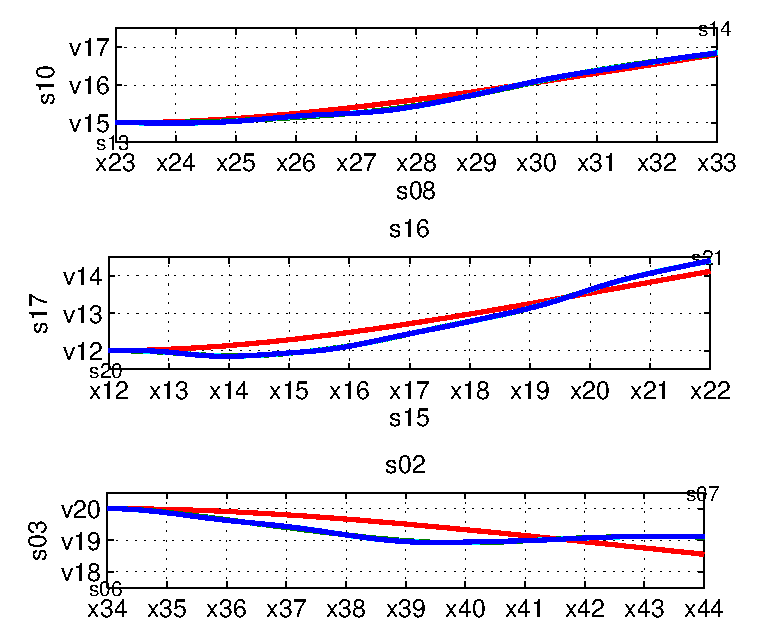
\includegraphics{./Figures/cantilevertimeevolution_t=all.eps}}%
\end{psfrags}%
%
% End cantilevertimeevolution_t=all.tex
\end{document}
% See http://www.mathworks.de/matlabcentral/fileexchange/loadFile.do?objectId=4638
% for recent versions of laprint.m.
%
% created by:           LaPrint version 3.16 (13.9.2004)
% created on:           14-Jan-2014 00:37:06
% eps bounding box:     15 cm x 10.0472 cm
% comment:              
%
\begin{psfrags}%
\psfragscanon%
%
% text strings:
\psfrag{s01}[t][t]{\color[rgb]{0,0,0}\setlength{\tabcolsep}{0pt}\begin{tabular}{c}{x}\end{tabular}}%
\psfrag{s02}[b][b]{\color[rgb]{0,0,0}\setlength{\tabcolsep}{0pt}\begin{tabular}{c}t=5 s\end{tabular}}%
\psfrag{s03}[b][b]{\color[rgb]{0,0,0}\setlength{\tabcolsep}{0pt}\begin{tabular}{c}displacement [m]\end{tabular}}%
\psfrag{s06}[][]{\color[rgb]{0,0,0}\setlength{\tabcolsep}{0pt}\begin{tabular}{c} \end{tabular}}%
\psfrag{s07}[][]{\color[rgb]{0,0,0}\setlength{\tabcolsep}{0pt}\begin{tabular}{c} \end{tabular}}%
\psfrag{s08}[t][t]{\color[rgb]{0,0,0}\setlength{\tabcolsep}{0pt}\begin{tabular}{c}{x}\end{tabular}}%
\psfrag{s09}[b][b]{\color[rgb]{0,0,0}\setlength{\tabcolsep}{0pt}\begin{tabular}{c}t=1 s\end{tabular}}%
\psfrag{s10}[b][b]{\color[rgb]{0,0,0}\setlength{\tabcolsep}{0pt}\begin{tabular}{c}displacement [m]\end{tabular}}%
\psfrag{s13}[][]{\color[rgb]{0,0,0}\setlength{\tabcolsep}{0pt}\begin{tabular}{c} \end{tabular}}%
\psfrag{s14}[][]{\color[rgb]{0,0,0}\setlength{\tabcolsep}{0pt}\begin{tabular}{c} \end{tabular}}%
\psfrag{s15}[t][t]{\color[rgb]{0,0,0}\setlength{\tabcolsep}{0pt}\begin{tabular}{c}{x}\end{tabular}}%
\psfrag{s16}[b][b]{\color[rgb]{0,0,0}\setlength{\tabcolsep}{0pt}\begin{tabular}{c}t=3 s\end{tabular}}%
\psfrag{s17}[b][b]{\color[rgb]{0,0,0}\setlength{\tabcolsep}{0pt}\begin{tabular}{c}displacement [m]\end{tabular}}%
\psfrag{s20}[][]{\color[rgb]{0,0,0}\setlength{\tabcolsep}{0pt}\begin{tabular}{c} \end{tabular}}%
\psfrag{s21}[][]{\color[rgb]{0,0,0}\setlength{\tabcolsep}{0pt}\begin{tabular}{c} \end{tabular}}%
%
% xticklabels:
\psfrag{x01}[t][t]{0}%
\psfrag{x02}[t][t]{0.1}%
\psfrag{x03}[t][t]{0.2}%
\psfrag{x04}[t][t]{0.3}%
\psfrag{x05}[t][t]{0.4}%
\psfrag{x06}[t][t]{0.5}%
\psfrag{x07}[t][t]{0.6}%
\psfrag{x08}[t][t]{0.7}%
\psfrag{x09}[t][t]{0.8}%
\psfrag{x10}[t][t]{0.9}%
\psfrag{x11}[t][t]{1}%
\psfrag{x12}[t][t]{0}%
\psfrag{x13}[t][t]{0.1}%
\psfrag{x14}[t][t]{0.2}%
\psfrag{x15}[t][t]{0.3}%
\psfrag{x16}[t][t]{0.4}%
\psfrag{x17}[t][t]{0.5}%
\psfrag{x18}[t][t]{0.6}%
\psfrag{x19}[t][t]{0.7}%
\psfrag{x20}[t][t]{0.8}%
\psfrag{x21}[t][t]{0.9}%
\psfrag{x22}[t][t]{1}%
\psfrag{x23}[t][t]{0}%
\psfrag{x24}[t][t]{0.1}%
\psfrag{x25}[t][t]{0.2}%
\psfrag{x26}[t][t]{0.3}%
\psfrag{x27}[t][t]{0.4}%
\psfrag{x28}[t][t]{0.5}%
\psfrag{x29}[t][t]{0.6}%
\psfrag{x30}[t][t]{0.7}%
\psfrag{x31}[t][t]{0.8}%
\psfrag{x32}[t][t]{0.9}%
\psfrag{x33}[t][t]{1}%
\psfrag{x34}[t][t]{0}%
\psfrag{x35}[t][t]{0.1}%
\psfrag{x36}[t][t]{0.2}%
\psfrag{x37}[t][t]{0.3}%
\psfrag{x38}[t][t]{0.4}%
\psfrag{x39}[t][t]{0.5}%
\psfrag{x40}[t][t]{0.6}%
\psfrag{x41}[t][t]{0.7}%
\psfrag{x42}[t][t]{0.8}%
\psfrag{x43}[t][t]{0.9}%
\psfrag{x44}[t][t]{1}%
%
% yticklabels:
\psfrag{v01}[r][r]{0}%
\psfrag{v02}[r][r]{0.1}%
\psfrag{v03}[r][r]{0.2}%
\psfrag{v04}[r][r]{0.3}%
\psfrag{v05}[r][r]{0.4}%
\psfrag{v06}[r][r]{0.5}%
\psfrag{v07}[r][r]{0.6}%
\psfrag{v08}[r][r]{0.7}%
\psfrag{v09}[r][r]{0.8}%
\psfrag{v10}[r][r]{0.9}%
\psfrag{v11}[r][r]{1}%
\psfrag{v12}[r][r]{0}%
\psfrag{v13}[r][r]{0.2}%
\psfrag{v14}[r][r]{0.4}%
\psfrag{v15}[r][r]{0}%
\psfrag{v16}[r][r]{0.2}%
\psfrag{v17}[r][r]{0.4}%
\psfrag{v18}[r][r]{-0.4}%
\psfrag{v19}[r][r]{-0.2}%
\psfrag{v20}[r][r]{0}%
%
% Figure:
\resizebox{12cm}{!}{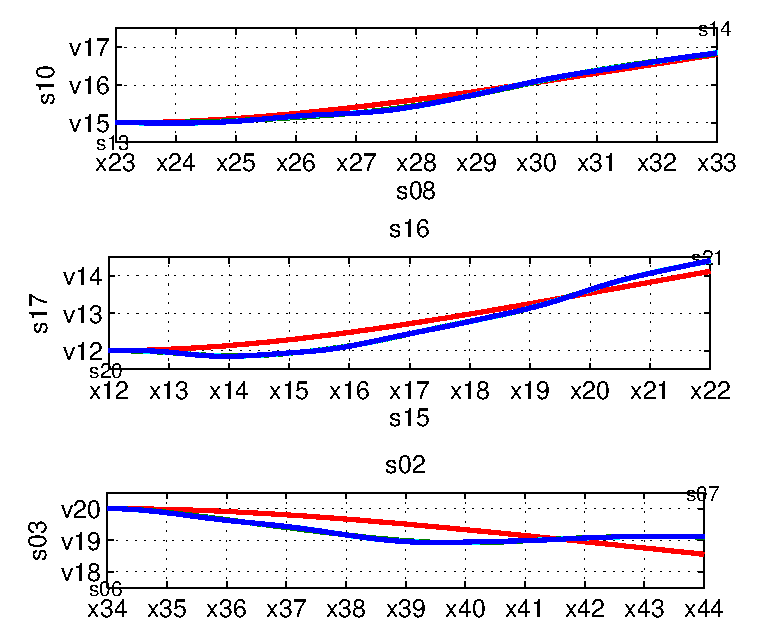
\includegraphics{./Figures/cantilevertimeevolution_t=all.eps}}%
\end{psfrags}%
%
% End cantilevertimeevolution_t=all.tex
\end{document}
% See http://www.mathworks.de/matlabcentral/fileexchange/loadFile.do?objectId=4638
% for recent versions of laprint.m.
%
% created by:           LaPrint version 3.16 (13.9.2004)
% created on:           14-Jan-2014 00:37:06
% eps bounding box:     15 cm x 10.0472 cm
% comment:              
%
\begin{psfrags}%
\psfragscanon%
%
% text strings:
\psfrag{s01}[t][t]{\color[rgb]{0,0,0}\setlength{\tabcolsep}{0pt}\begin{tabular}{c}{x}\end{tabular}}%
\psfrag{s02}[b][b]{\color[rgb]{0,0,0}\setlength{\tabcolsep}{0pt}\begin{tabular}{c}t=5 s\end{tabular}}%
\psfrag{s03}[b][b]{\color[rgb]{0,0,0}\setlength{\tabcolsep}{0pt}\begin{tabular}{c}displacement [m]\end{tabular}}%
\psfrag{s06}[][]{\color[rgb]{0,0,0}\setlength{\tabcolsep}{0pt}\begin{tabular}{c} \end{tabular}}%
\psfrag{s07}[][]{\color[rgb]{0,0,0}\setlength{\tabcolsep}{0pt}\begin{tabular}{c} \end{tabular}}%
\psfrag{s08}[t][t]{\color[rgb]{0,0,0}\setlength{\tabcolsep}{0pt}\begin{tabular}{c}{x}\end{tabular}}%
\psfrag{s09}[b][b]{\color[rgb]{0,0,0}\setlength{\tabcolsep}{0pt}\begin{tabular}{c}t=1 s\end{tabular}}%
\psfrag{s10}[b][b]{\color[rgb]{0,0,0}\setlength{\tabcolsep}{0pt}\begin{tabular}{c}displacement [m]\end{tabular}}%
\psfrag{s13}[][]{\color[rgb]{0,0,0}\setlength{\tabcolsep}{0pt}\begin{tabular}{c} \end{tabular}}%
\psfrag{s14}[][]{\color[rgb]{0,0,0}\setlength{\tabcolsep}{0pt}\begin{tabular}{c} \end{tabular}}%
\psfrag{s15}[t][t]{\color[rgb]{0,0,0}\setlength{\tabcolsep}{0pt}\begin{tabular}{c}{x}\end{tabular}}%
\psfrag{s16}[b][b]{\color[rgb]{0,0,0}\setlength{\tabcolsep}{0pt}\begin{tabular}{c}t=3 s\end{tabular}}%
\psfrag{s17}[b][b]{\color[rgb]{0,0,0}\setlength{\tabcolsep}{0pt}\begin{tabular}{c}displacement [m]\end{tabular}}%
\psfrag{s20}[][]{\color[rgb]{0,0,0}\setlength{\tabcolsep}{0pt}\begin{tabular}{c} \end{tabular}}%
\psfrag{s21}[][]{\color[rgb]{0,0,0}\setlength{\tabcolsep}{0pt}\begin{tabular}{c} \end{tabular}}%
%
% xticklabels:
\psfrag{x01}[t][t]{0}%
\psfrag{x02}[t][t]{0.1}%
\psfrag{x03}[t][t]{0.2}%
\psfrag{x04}[t][t]{0.3}%
\psfrag{x05}[t][t]{0.4}%
\psfrag{x06}[t][t]{0.5}%
\psfrag{x07}[t][t]{0.6}%
\psfrag{x08}[t][t]{0.7}%
\psfrag{x09}[t][t]{0.8}%
\psfrag{x10}[t][t]{0.9}%
\psfrag{x11}[t][t]{1}%
\psfrag{x12}[t][t]{0}%
\psfrag{x13}[t][t]{0.1}%
\psfrag{x14}[t][t]{0.2}%
\psfrag{x15}[t][t]{0.3}%
\psfrag{x16}[t][t]{0.4}%
\psfrag{x17}[t][t]{0.5}%
\psfrag{x18}[t][t]{0.6}%
\psfrag{x19}[t][t]{0.7}%
\psfrag{x20}[t][t]{0.8}%
\psfrag{x21}[t][t]{0.9}%
\psfrag{x22}[t][t]{1}%
\psfrag{x23}[t][t]{0}%
\psfrag{x24}[t][t]{0.1}%
\psfrag{x25}[t][t]{0.2}%
\psfrag{x26}[t][t]{0.3}%
\psfrag{x27}[t][t]{0.4}%
\psfrag{x28}[t][t]{0.5}%
\psfrag{x29}[t][t]{0.6}%
\psfrag{x30}[t][t]{0.7}%
\psfrag{x31}[t][t]{0.8}%
\psfrag{x32}[t][t]{0.9}%
\psfrag{x33}[t][t]{1}%
\psfrag{x34}[t][t]{0}%
\psfrag{x35}[t][t]{0.1}%
\psfrag{x36}[t][t]{0.2}%
\psfrag{x37}[t][t]{0.3}%
\psfrag{x38}[t][t]{0.4}%
\psfrag{x39}[t][t]{0.5}%
\psfrag{x40}[t][t]{0.6}%
\psfrag{x41}[t][t]{0.7}%
\psfrag{x42}[t][t]{0.8}%
\psfrag{x43}[t][t]{0.9}%
\psfrag{x44}[t][t]{1}%
%
% yticklabels:
\psfrag{v01}[r][r]{0}%
\psfrag{v02}[r][r]{0.1}%
\psfrag{v03}[r][r]{0.2}%
\psfrag{v04}[r][r]{0.3}%
\psfrag{v05}[r][r]{0.4}%
\psfrag{v06}[r][r]{0.5}%
\psfrag{v07}[r][r]{0.6}%
\psfrag{v08}[r][r]{0.7}%
\psfrag{v09}[r][r]{0.8}%
\psfrag{v10}[r][r]{0.9}%
\psfrag{v11}[r][r]{1}%
\psfrag{v12}[r][r]{0}%
\psfrag{v13}[r][r]{0.2}%
\psfrag{v14}[r][r]{0.4}%
\psfrag{v15}[r][r]{0}%
\psfrag{v16}[r][r]{0.2}%
\psfrag{v17}[r][r]{0.4}%
\psfrag{v18}[r][r]{-0.4}%
\psfrag{v19}[r][r]{-0.2}%
\psfrag{v20}[r][r]{0}%
%
% Figure:
\resizebox{12cm}{!}{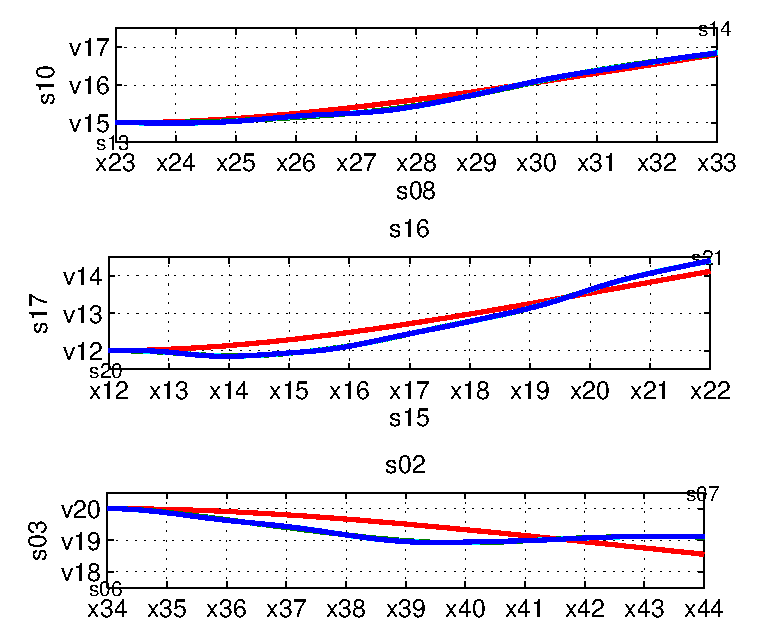
\includegraphics{./Figures/cantilevertimeevolution_t=all.eps}}%
\end{psfrags}%
%
% End cantilevertimeevolution_t=all.tex

\end{subfigure}\\
\\
\\
\begin{subfigure}[b]{1\textwidth}
\centering
\includegraphics[width=0.4\textwidth]{./Figures/cantilevertimeevolution_legend}
\end{subfigure}
\caption{Plot of cantilever beam for t=1, t=3 and t=5 s. }
\label{fig:cantilevertimeevolution}
\end{figure}
\bibliographystyle{plain}
\bibliography{biblio}

\end{document}          


